% \iffalse meta-comment
% !TEX program = pdfLaTeX
% 
% ------------------------------------------------------------------------------
% Beamer theme cuerna, version 1.1
% Copyright (C) 2016 by Geri Ochoa 
% email: geri@bluesimplex.com
% github: https://github.com/geriom/beamercuerna
% my web site: bluesimplex.com
% 
% This work may be distributed and/or modified under the conditions of the LaTeX
% Project Public License, either version 1.3 of this license or (at your option)
% any later version. The latest version of this license is in
% http://www.latex-project.org/lppl.txt and version 1.3 or later is part of all
% distributions of LaTeX version 2005/12/01 or later.
% ------------------------------------------------------------------------------
% 
% \fi
% 

% \iffalse
%<*driver>
\ProvidesFile{beamercuerna.dtx}[2016/09/18 v1.1 beamer theme cuerna]
\documentclass{ltxdoc}
\EnableCrossrefs
\CodelineIndex
\RecordChanges

\OnlyDescription
\begin{document}
  \DocInput{beamercuerna.dtx}
  \PrintChanges
  \PrintIndex
\end{document}
%</driver>

% \fi

% \CheckSum{0}
%
% \changes{v1.0}{2014/10/22}{Initial version}
%
% \GetFileInfo{beamercuerna.dtx}
%
% \DoNotIndex{\newcommand, \newenvironment}
%
% \title{The \textsf{beamercuerna} beamer theme\thanks{This document
% corresponds to \textsf{beamercuerna}~\fileversion, date \filedate.}}
% \author{Geri Ochoa \\ \texttt{ger@bluesimplex.com}}
%
% \maketitle
%
% \section{Introduction}
% Here I'm going to give a brief intro

% \section{Usage}
% Here I will provide examples
%
% \StopEventually{}
% \begin{macrocode}
%<*cuerna>
\mode<presentation>

%Required packages
\RequirePackage{tikz}
\RequirePackage{graphicx}
\RequirePackage{amssymb}
\RequirePackage{xcolor}
\RequirePackage{lmodern}
\RequirePackage[absolute, overlay]{textpos}

%Color config files
\usecolortheme{Cuerna}
\useinnertheme{Cuerna}
\useoutertheme{Cuerna}


\setbeamertemplate{navigation symbols}{}
\setbeamertemplate{blocks}[rounded][shadow=true]

\mode<all>
%</cuerna>
%
%
%<*inner>
\mode<presentation>

%This draws the background
\setbeamertemplate{background}{
  \begin{tikzpicture}[espiral/.style={thick,color=edgescolor}]
    \useasboundingbox (0,0) rectangle(\the\paperwidth,\the\paperheight);
    \fill[color=edgescolor] (0,0) rectangle(\the\paperwidth, \the\paperheight);
    \fill[color=squarecolor] (0,0) rectangle(0.59\paperwidth, \the\paperheight);
    \draw[espiral] (0,0) .. controls +(up:0.5\paperheight) and (0.3\paperwidth,  \the\paperheight) .. (0.59\paperwidth,\the\paperheight);
    \fill[color=squarecolor] (0.60\paperwidth,0.41\paperheight) rectangle(\the\paperwidth, \the\paperheight);
    \draw[espiral] (0.60\paperwidth,\paperheight) .. controls +(right:0.3\paperwidth) and (\paperwidth, 0.61\paperheight) .. (\the\paperwidth, 0.41\paperheight);
    \fill[color=squarecolor] (0.77\paperwidth,0) rectangle(\the\paperwidth, 0.40\paperheight);
    \draw[espiral] (\paperwidth,0.4\paperheight) .. controls +(down:0.2\paperwidth) and (0.88\paperwidth, 0) .. (0.77\paperwidth, 0);
    \fill[color=squarecolor] (0.6\paperwidth,0) rectangle(0.76\paperwidth, 0.23\paperheight);
    \draw[espiral] (0.76\paperwidth,0) .. controls +(left:0.08\paperwidth) and (0.6\paperwidth, 0.12\paperheight) .. (0.6\paperwidth, 0.23\paperheight);
    \fill[color=squarecolor] (0.6\paperwidth, 0.24\paperheight) rectangle(0.69\paperwidth, 0.4\paperheight);
    \draw[espiral] (0.6\paperwidth,0.24\paperheight) .. controls +(up:0.08\paperheight) and (0.64\paperwidth, 0.4\paperheight) .. (0.69\paperwidth, 0.4\paperheight);
    \fill[color=squarecolor] (0.70\paperwidth, 0.31\paperheight) rectangle(0.76\paperwidth, 0.40\paperheight);
    \draw[espiral] (0.7\paperwidth,0.4\paperheight) .. controls +(right:0.03\paperheight) and (0.76\paperwidth, 0.35\paperheight) .. (0.76\paperwidth, 0.31\paperheight);
    \fill[color=squarecolor] (0.72\paperwidth, 0.24\paperheight) rectangle(0.76\paperwidth, 0.3\paperheight);
    \draw[espiral] (0.76\paperwidth,0.3\paperheight) .. controls +(down:0.03\paperheight) and (0.74\paperwidth, 0.24\paperheight) .. (0.72\paperwidth, 0.24\paperheight);
    \fill[color=squarecolor] (0.70\paperwidth, 0.24\paperheight) rectangle(0.71\paperwidth, 0.28\paperheight);
    \draw[espiral] (0.71\paperwidth,0.24\paperheight) .. controls +(left:0.005\paperwidth) and (0.7\paperwidth, 0.26\paperheight) .. (0.7\paperwidth, 0.28\paperheight);
    \ifnum\thepage>1\relax%
    \fill[white, opacity=1] (0,0) rectangle(\the\paperwidth, \the\paperheight);
    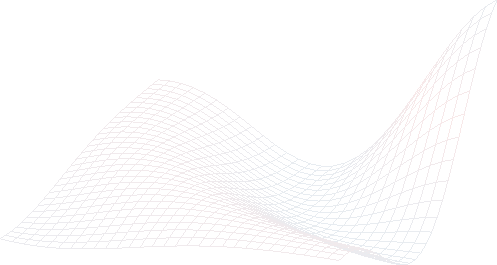
\includegraphics[width=\paperwidth, height=0.8\paperheight,
    angle=35]{fondo.pdf}
    \fi
  \end{tikzpicture}
}

\setbeamerfont{date}{size=\large, shape=\upshape}
\setbeamerfont{title}{size=\huge, shape=\mdseries}
\setbeamerfont{institute}{size=\tiny, shape=\itshape}

%Creates the title page contents
\defbeamertemplate*{title page}{Cuerna}[1][]
{
  \begin{textblock}{9}(0.2,2.5)
    \begin{beamercolorbox}[center,sep=1pt,#1]{title page header}
      \usebeamerfont{title}\inserttitle\par%
    \end{beamercolorbox}
  \end{textblock}
  \vskip4.5cm%
  \begin{beamercolorbox}[wd=6cm,leftskip=0cm,#1]{author}
    \usebeamerfont{date}\insertauthor%
  \end{beamercolorbox}
  \vskip0.1cm%
  \begin{beamercolorbox}[wd=6cm, #1]{institute}
    \usebeamerfont{institute}\insertinstitute
  \end{beamercolorbox}


  \begin{textblock}{6}(9.3,5)
    \begin{beamercolorbox}[right]{date}
      \usebeamerfont{date}\insertdate%
    \end{beamercolorbox}
  \end{textblock}

  \begin{textblock}{4}(12.9,11.8)
    \insertlogo
  \end{textblock}
  \vfill
}

%Lists and the table of contents
\setbeamertemplate{items}[triangle]
\setbeamertemplate{sections/subsections in toc}[square]

\mode<all>
%</inner>
%
%
%<*outer>
\mode<presentation>

\setbeamerfont{sectiontitle}{size=\huge, shape=\scshape}

%Title bar
\defbeamertemplate*{frametitle}{Cuerna}[1][]
{
  \vskip0.2cm
  \begin{beamercolorbox}[right]{sectiontitle}
    \usebeamerfont{date}\insertsection
  \end{beamercolorbox}
  \vskip-0.2cm
  \definecolor{imred}{HTML}{BD2026}
  \definecolor{imyellow}{HTML}{FCED27}
  \definecolor{imorange}{HTML}{F6B419}
  \begin{beamercolorbox}[wd=\paperwidth,ht=1.9cm]{frametitle}
    \begin{tikzpicture}
      \useasboundingbox (0,0) rectangle(\the\paperwidth,1.4);
      {\node[anchor=west, white] at (0.4, 0.8){\insertlogo};}
      \fill[squarecolor](2.45, 0.3) rectangle(\paperwidth,1.4);
      \ifx\insertframesubtitle\@empty%
      {\node[anchor=west, white, font=\large] at (3.0,0.82){\insertframetitle};}
      \else%
      {\node[anchor=west, white, font=\large] at (3.0, 1.02){\insertframetitle};%
      \node[anchor=west, white, font=\small] at (3.0, 0.63){\insertframesubtitle};}%
      \fi
    \end{tikzpicture}
  \end{beamercolorbox}
  \vskip-0.5cm
}

%Prevents the logo from beign added to every slide
\defbeamertemplate*{sidebar right}{sidebar theme}
{%
  \vfill%
  \llap{\usebeamertemplate***{navigation symbols}\hskip0.1cm}%
\vskip2pt}

\mode<all>
%</outer>
%
%
%<*default>
\mode<presentation>

\definecolor{edgescolor}{HTML}{4DA6FF}
\definecolor{squarecolor}{HTML}{002B36}

%Colours to use in some elements
\setbeamercolor*{title page header}{fg=white}
\setbeamercolor*{author}{fg=white}
\setbeamercolor*{date}{fg=white}
\setbeamercolor*{institute}{fg=white}
\setbeamercolor*{sectiontitle}{fg=black}

%Item list colour
\setbeamercolor*{item}{fg=squarecolor}

%Theorem box colour
\setbeamercolor{block title}{use=structure,fg=white,bg=squarecolor}

\mode<all>
%</default>
%
%
%<*bluesimplex>
\mode<presentation>

\definecolor{edgescolor}{HTML}{3469CC}
\definecolor{to use in}{HTML}{282d33}

%Colours to use in some elements
\setbeamercolor*{title page header}{fg=white}
\setbeamercolor*{author}{fg=white}
\setbeamercolor*{date}{fg=white}
\setbeamercolor*{institute}{fg=white}
\setbeamercolor*{sectiontitle}{fg=black}

%Item list colour
\setbeamercolor*{item}{fg=squarecolor}

%Theorem box colour
\setbeamercolor{block title}{use=structure,fg=white,bg=squarecolor}

\mode<all>
%</bluesimplex>
%
%
%<*brick>
\mode<presentation>

\definecolor{edgescolor}{HTML}{3469CC}
\definecolor{to use in}{HTML}{282d33}

%Colours to use in some elements
\setbeamercolor*{title page header}{fg=white}
\setbeamercolor*{author}{fg=white}
\setbeamercolor*{date}{fg=white}
\setbeamercolor*{institute}{fg=white}
\setbeamercolor*{sectiontitle}{fg=black}

%Item list colour
\setbeamercolor*{item}{fg=squarecolor}

%Theorem box colour
\setbeamercolor{block title}{use=structure,fg=white,bg=squarecolor}

\mode<all>
%</brick>
%
%
%<*lettuce>
\mode<presentation>

\definecolor{edgescolor}{HTML}{757575}
\definecolor{squarecolor}{HTML}{3B5323}

%Colours to use in some elements
\setbeamercolor*{title page header}{fg=white}
\setbeamercolor*{author}{fg=white}
\setbeamercolor*{date}{fg=white}
\setbeamercolor*{institute}{fg=white}
\setbeamercolor*{sectiontitle}{fg=black}

%Item list colour
\setbeamercolor*{item}{fg=squarecolor}

%Theorem box colour
\setbeamercolor{block title}{use=structure,fg=white,bg=squarecolor}

\mode<all>
%</lettuce>

% \end{macrocode}

%\Finale
